\chapter{Spazi Metrici}

\section{Preliminari}
% TODO definzione campo

\begin{definition}[Spazio Vettoriale]
	Siano $K$ un \textbf{campo} e $V$ un \textbf{insieme}. Si dice che \textbf{Spazio Vettoriale} sul campo $K$ se sono definite due operazioni:
	\begin{enumerate}
		\item \textbf{Somma}, operazione interna binaria
		\item \textbf{Prodotto per scalari} operazione esterna
	\end{enumerate}
	\begin{note}
		Questa definizione è stata riportata per ricordare il concetto, si consiglia la consultazione di un libro di Algebra Lineare per una definizione più precisa.
	\end{note}
\end{definition}

\begin{definition}[Spazio Metrico]
	\label{def:sp_metrico}
	Si dice Spazio Metrico $(X,d)$ un insieme $X$ non vuoto in cui sia definita una \textbf{distanza} (o \textbf{metrica}), vale a dire una funzione $d: X \times X \mapsto \R$ con le seguenti proprietà:
	\begin{enumerate}
		\item $d(x,y) \geq 0 \quad \forall x,y \in X$
		\item $d(x,y) = 0 \quad \forall x,y \in X \iff x=y$
		\item $d(x,y) = d(y,x) \quad \forall x,y \in X$ \quad(\textit{simmetria})
		\item $d(x,z) \leq d(x,y)+d(y,z) \quad \forall x,y,z\in X$ \quad(\textit{disuguaglianza triangolare})
	\end{enumerate}
	\begin{note}
		D'ora in poi, quando si userà $d$ come metrica, dove non diversamente specificato, si intenderà la \textbf{Metrica Euclidea} di \hyperref[ex:dist_eucl]{\cref*{ex:metriche} (\nameref*{ex:metriche})}
	\end{note}
\end{definition}

Unendo le due definizioni si giunge naturalmente a
\begin{definition}[Spazio Vettoriale Metrico]
	Uno Spazio Vettoriale Metrico è uno spazio vettoriale $V$ su cui è definito un prodotto scalare $<\cdot,\cdot·>$ definito positivo, la sua \textbf{metrica}.
	\begin{note}
		Analogamente si definisce il Sottospazio Vettoriale Metrico
	\end{note}
\end{definition}

\begin{definition}[Metrica Indotta]
	\label{def:metr_indotta}
	Siano $(X,d)$ spazio metrico e $S \subseteq X$ con $S \neq \emptyset$\\
	Allora $d_{|S} = d_{|S \times S}$ è una metrica su $S$, cioè la metrica $d_{|S}$ è la \textbf{metrica indotta}, definita come la \textbf{restrizione} della metrica $d$ ai soli elementi di $S$. Si definisce formalmente come
	$$\funcdef{d_{|S}}{S \times S}{\R}{(x,y)}{d(x,y)}$$
\end{definition}

\begin{definition}[Sottospazio Metrico]
	Siano $(X,d)$ spazio metrico e $S \subseteq X$ con $S \neq \emptyset$\\
	Allora $(S,d_{|S})$ con la \fullref{def:metr_indotta} è a sua volta Spazio Metrico ed è chiamato \textbf{Sottospazio Metrico di $(X,d)$}
	\begin{proof}
		La $d_{|S}$, essendo restrizione della metrica $d$, rispetta ancora tutti i punti della \fullref{def:sp_metrico}.
	\end{proof}
\end{definition}

\begin{proposition}
	\label{prop:subspace_condition}
	Sia $(V)$ uno spazio vettoriale metrico sul campo $K$ e sia $\emptyset \neq U \subseteq V$. Il sottoinsieme $U$ è un sottospazio vettoriale metrico se, e soltanto se, sono verificate le seguenti condizioni:
	\begin{enumerate}
		\item $\forall \mathbf{u}, \mathbf{u'} \in U \quad \mathbf{u} + \mathbf{u'} \in U$
		\item $\forall \lambda \in K,\; \forall \mathbf{u} \in U \quad \lambda \cdot \mathbf{u} \in U$
	\end{enumerate}
	\begin{proof}
		Non richiesta, analoga a quella per Spazi Vettoriali reperibile in un libro di Algebra Lineare
	\end{proof}
\end{proposition}

\begin{example}[Esempi di Metriche]
	\label{ex:metriche}
	Si dimostri che le seguenti funzioni sono distanze:
	\begin{note}
		Si noti che alcuni degli esempi sottostanti sono relativi a metriche trattate molto più avanti e dunque potrebbe essere conveniente ignorarli temporaneamente per tornare qui quando saranno stati fatti i successivi argomenti.
	\end{note}
	\begin{enumerate}
		\item $X=\R^2,\quad d(x,y) = d\bigl((x_1,x_2),(y_1,y_2)\bigr) = \sqrt{(y_1-x_1)^2+(y_2-x_2)^2}$ \hfill {\footnotesize\textbf{Metrica Euclidea in $\R^2$}}
			\begin{enumerate}[label=\arabic*]
				\item $d(x,y) \geq 0$ è verificata poiché l'argomento della radice è sempre positivo o al più nullo essendo una somma di quadrati, e la radice mantiene la positività.
				\item $d(x,y) = 0 \iff x = y$
					\begin{align*}
						d = 0 &\iff \sqrt{(y_1-x_1)^2+(y_2-x_2)^2} = 0\\
						&\iff (y_1-x_1)^2+(y_2-x_2)^2 = 0\\
						&\iff \begin{cases}
							(y_1-x_1)^2=0\\
							(y_2-x_2)^2=0\\
						\end{cases}\\
						&\iff
						\begin{cases}
							y_1=x_1\\
							y_2=x_2\\
						\end{cases}\\
						&\iff (x_1,x_2)=(y_1,y_2)
					\end{align*}
				\item $d(x,y) = d(y,x)$ invertendo le coordinate di $x$ con quelle di $y$ la somma non cambia, quindi la simmetria è rispettata
					$$d\bigl((x_1,x_2),(y_1,y_2)\bigr) \bigr) = \sqrt{(y_1-x_1)^2+(y_2-x_2)^2} = \sqrt{(y_2-x_2)^2+(y_1-x_1)^2} = d\bigl((y_1,y_2),(x_1,x_2)\bigr)$$
				\item $d(x,y) \leq d(x,z) + d(z,y)$ da \fullref{prop:dist_sp_norm}, la metrica indotta dalla norma (\fullref{def:norma}), applicata ad $\R^2$ è
					$$\norm{x - y} = \sqrt{(y_1-x_1)^2+(y_2-x_2)^2}$$
					che corrisponde alla metrica in oggetto. Dunque, grazie alle proprietà dell'operatore $\norm{\;\cdot\;}$ (nello specifico la \textit{disuguaglianza triangolare}), si ottiene
					$$d(x,y) = \norm{x-y} = \norm{(x-z) + (z-y)} \leq \norm{x-z} + \norm{z-y} = d(x,z) + d(z,y)$$
					\begin{center}
						\begin{tikzpicture}[scale=0.5]
						\draw (0,0) node[anchor=north east]{$x=(x_1,x_2)$}
							-- (4,4) node[anchor=south]{$y=(y_1,y_2)$}
							-- (4,0) node[anchor=north west]{$z=(z_1,z_2)$}
							-- cycle;
						\end{tikzpicture}
					\end{center}
			\end{enumerate}
		\item $X=\R,\quad d(x,y)=\abs{y-x}$ \hfill {\footnotesize\textbf{Metrica Euclidea in $\R$}}
			\begin{enumerate}[label=\arabic*.]
				\item $d(x,y) \geq 0$ per definizione valore assoluto
				\item $d(x,y) = 0 \iff x = y$ perché $\abs{\;\cdot\;} = 0 \iff \cdot\; = 0$ per definizione valore assoluto
				\item $d(x,y)=d(y,x)$ perché $\abs{x - y} = \abs{y - x}$ per definizione valore assoluto
				\item $d(x,y) \leq d(x,z) + d(z,y)$ in quanto
					$$d(x,y) = \abs{x-y} = \abs{x-z+z-y} \leq \abs{x-z} + \abs{z-y} = d(x,z) + d(z,y)$$
			\end{enumerate}
		\item $X=\R^n \;\; \text{con}\; x=(x_1,\ldots,x_n),\; y=(y_1,\ldots,y_n),\quad d(x,y)=\sqrt{\sum\limits_{i=1}^{n}{\left(y_i-x_i\right)}^2}$ \hfill {\footnotesize\textbf{Metrica Euclidea in $\R^n$}} \label{ex:dist_eucl}\\
			Analogo al primo esempio
		\item $X\ne \emptyset,\quad d(x,y)=
			\begin{cases}
				\begin{matrix}
					0&&x=y\\
					1&&x \ne y
				\end{matrix}
			\end{cases}$ \hfill {\footnotesize\textbf{Metrica Discreta}}\label{ex:dist_discr}
			\begin{enumerate}[label=\arabic*.]
				\item $d(x,y) \geq 0$ per definizione
				\item $d(x,y) = 0 \iff x = y$ per definizione
				\item $d(x,y)=d(y,x)$ per definizione (sia che $x = y$, sia che $x \neq y$)
				\item $d(x,y) \leq d(x,z) + d(z,y)$ perché $d(x,z) + d(z,y)$ può essere:
					\begin{itemize}
						\item $0$ se $x = y = z$, ma in questo caso anche $d(x,y) = 0$
						\item $1$ se $x = y \neq z$ o $x \neq y = z$, ma in questo caso $d(x,y) \leq 1$
						\item $2$ se $x \neq y \neq z$, quindi sicuramente $d(x,y) \leq d(x,z) + d(z,y)$
					\end{itemize}
			\end{enumerate}
		\item $X=\cntclass{0}(\realintervalclose{a}{b},\R)\;a,b\in\R,\;a<b \quad d_\infty(f,g) = \sup\limits_{x\in\realintervalclose{a}{b}}\abs{g(x)-f(x)}$ \hfill
			{\footnotesize
				\begin{tabular}{c}
					\textbf{Distanza della Convergenza Infinita}\\
					o\\
					\textbf{Distanza della Convergenza Uniforme}
				\end{tabular}
			}\label{ex:dim_dist_conv_unif}
			\begin{note}
				La metrica viene trattata in \fullref{def:conv_unif}
			\end{note}
			\begin{note}
				$X$ contiene infiniti elementi (funzioni)
			\end{note}
			\begin{center}
				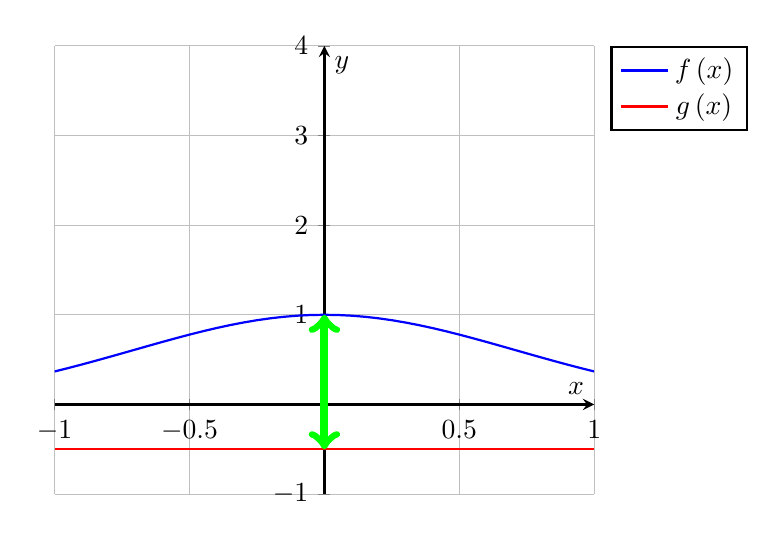
\begin{tikzpicture}[scale=1]
					\begin{axis}[
						xlabel={$x$},ylabel={$y$},
						axis lines=middle,
						samples=41,grid,thick,
						domain=-1:1,
						ymin=-1,ymax=4,
						legend pos=outer north east ]
						\addplot+[no marks] {e^-(abs(x*x))}; \addlegendentry{$f\left( x \right)$}
						\addplot+[no marks] {-0.5}; \addlegendentry{$g\left( x \right)$}
						\draw[<->,line width=1mm, color=green] (axis cs:0,-0.5) -- (axis cs:0,1);
					\end{axis}
				\end{tikzpicture}
			\end{center}
			\begin{enumerate}[label=\arabic*.]
				\item $d(x,y) \geq 0$ per definizione, il valore è sicuramente appartenente a $\realintervalclose{0}{+\infty}$, ma $+\infty$ non è un valore accettabile, in quanto la metrica è definita come funzione a valori in $\R$ e $+\infty \notin \R$. D'alto canto, si nota che $X$ è definito come l'insieme delle funzioni continue definite su un intervallo \textbf{chiuso e limitato} a valori in $\R$ ($\cntclass{0}(\realintervalclose{a}{b},\R)$). Questa definizione permette di applicare il \fullref{teo:weier} ed avere la certezza che esista $\sup$ finito.
				\item $d(x,y) = 0 \iff x = y$ per definizione, $d_\infty(f,g) = 0 \iff \sup\limits_{x\in\realintervalclose{a}{b}}\abs{g(x)-f(x)} = 0$, cioè se e solo se le due funzioni hanno lo stesso dominio e, per ogni punto di esso, la stessa immagine.
				\item $d(x,y)=d(y,x)$ semplicmente $d_{\infty}(f,g) = \sup\limits_{x\in\realintervalclose{a}{b}}\abs{f-g} = \sup\limits_{x\in\realintervalclose{a}{b}}\abs{g-f} = d_{\infty}(g,f)$
				\item $d(x,y) \leq d(x,z) + d(z,y)$ dalla disuguaglianza triangolare per $\abs{\;\cdot\;}$ si ottiene
					$$\abs{g(x)-f(x)}\le\abs{g(x)-h(x)}+\abs{h(x)-f(x)}$$
					Applicando il sup la disuguaglianza resta vera.
			\end{enumerate}
			\begin{note}
				Si sottolinea che queste conclusioni sono valide finché $\realintervalclose{a}{b}$ chiuso e limitato, altrimenti non varrebbe più il \fullref{teo:weier} necessario per il punto 1. % TODO Serve un controesempio
			\end{note}
		\item $X=\R^2$, $d$ distanza Euclidea e $P$ punto arbitrario\newline
			$\quad d_P(x,y)=
			\begin{cases}
				\begin{array}{ll}
					0 & \text{se } x = y\\
					d(x,P) + d(P,y) & \text{se } x \neq y
				\end{array}
			\end{cases}$ \hfill
			{\footnotesize
				\begin{tabular}{c}
					\textbf{Distanza di Parigi}\\
					o\\
					\textbf{Distanza Ferroviaria Francese}
				\end{tabular}
			} \label{ex:dist_parigi}
			\begin{enumerate}[label=\arabic*.]
				\item $d(x,y) \geq 0$ per definizione
				\item $d(x,y) = 0 \iff x = y$ per definizione
				\item $d(x,y)=d(y,x)$ essendo bassata sulla metrica Euclidea
				\item $d(x,y) \leq d(x,z) + d(z,y)$ essendo bassata sulla metrica Euclidea
			\end{enumerate}
		\item $X=\cntclass{0}(\realintervalclose{a}{b},\R)\;a,b\in\R,\;a<b \quad d_2(f,g) = \sqrt{\int_a^b\left[g(x)-f(x)\right]^2 \integrald{x}}$ \hfill {\footnotesize\textbf{Distanza Quadratica}}
		\label{ex:dim_dist_quadratica}
			\begin{note}
				La metrica viene trattata in \fullref{def:dist_quadratica}
			\end{note}
			\begin{enumerate}[label=\arabic*.]
				\item $d(x,y) \geq 0$ per definizione, essendo integrale di un valore positivo (quadrato) tra estremi ordinati ($a<b$ per ipotesi)
				\item $d(x,y) = 0 \iff x = y$ Per definizione della metrica, $d_2(f,g) = 0 \iff \sqrt{\int_a^b\left[g(x)-f(x)\right]^2 \integrald{x}} = 0$, cioè se e solo se le due funzioni hanno lo stesso dominio e, per ogni punto di esso, la stessa immagine.
				\item $d(x,y)=d(y,x)$ semplicmente $d_2(f,g) = \sqrt{\int_a^b\left[g(x)-f(x)\right]^2 \integrald{x}} = \sqrt{\int_a^b\left[f(x)-g(x)\right]^2 \integrald{x}} = d_2(g,f)$
				\item $d(x,y) \leq d(x,z) + d(z,y)$ ... % TODO Spiegare questo punto
			\end{enumerate}
	\end{enumerate}
\end{example}

\begin{definition}[Norma]
	\label{def:norma}
	Dato uno spazio vettoriale $V$ sul campo $\mathbb{K}$, si definisce \textbf{norma} una funzione $\norm{\cdot}:V\mapsto\R$ con le proprietà:
	\begin{enumerate}
		\item $\norm{x} \geq 0 \quad \forall x\in V$
		\item $\norm{x}=0 \iff x = 0 \quad \forall x\in V$
		\item $\norm{x+y} \leq \norm{x}+\norm{y} \quad \forall x,y\in V$
		\item $\norm{\lambda x} = \abs{\lambda} \cdot \norm{x} \quad \forall x\in V,\lambda\in\mathbb{K}$
	\end{enumerate}
	\begin{note}
		La funzione Norma associa dunque ad un vettore di qualsiasi dimensione uno scalare, fornendo (anche) una metrica per ordinare vettori tra loro.
	\end{note}
\end{definition}
\begin{definition}[Spazio Normato]
	Uno spazio normato è uno spazio vettoriale $V$ sul campo $\mathbb{K}$ \textbf{in cui è definita una norma}.
	\begin{note}
		Nel seguito verranno considerati esclusivamente spazi vettoriali su $\R$ o su $\C$, cioè $\mathbb{K} = \R$ o $\mathbb{K} = \C$
	\end{note}
\end{definition}

\begin{example}[Esempi di Spazi Normati]\leavevmode\vspace*{-\baselineskip}
	\begin{enumerate}
		\item $\R$ con $\norm{x} = \abs{x}$
		\item $\C$ con $\norm{x} = \abs{x}$
		\item $\R^n$ con $\norm{x} = \sqrt{\sum\limits_{i=1}^{n}x_i^2}$
		\item $\cntclass{0}(\realintervalclose{0}{1};\R)$ con $\norm{f} = \sup\limits_{x \in \realintervalclose{0}{1}} \abs{f(x)}$
	\end{enumerate}
\end{example}

\begin{proposition}[Metrica Indotta da una Norma]
	\label{prop:dist_sp_norm}
	Sia $V$ uno spazio normato. Allora $(V,d)$ è uno spazio metrico con la distanza
	$$d(x,y) = \norm{y-x}$$
	ed inoltre la distanza così definita è:
	\begin{enumerate}
		\item Invariante per traslazioni:
			$$\forall x,y,z \in V,\; d(x,y) = d(x+z, y+z)$$
		\item Positivamente omogenea:
			$$\forall x,y \in V\: \text{e} \forall \lambda \in \R,\; d(\lambda x, \lambda y) = \abs{\lambda}d(x,y)$$
	\end{enumerate}
	\begin{proof}
		~
		\begin{enumerate}
			\item $d(x,y) = d(x+z, y+z) = \norm{y+z-x-z} = \norm{y-x} = d(x,y)$
			\item Con la proprietà 4 della \fullref{def:norma}
			$$d(\lambda x, \lambda y) = \norm{\lambda y - \lambda x} = \norm{\lambda (y - x)} = \abs{\lambda} \norm{y - x} = \abs{\lambda}d(x,y)$$
		\end{enumerate}
	\end{proof}
	\begin{note}
		Nel caso in cui $V = \R^n$, la metrica indotta è ovviamente la \textbf{Metrica Euclidea} di \hyperref[ex:dist_eucl]{\cref*{ex:metriche} (\nameref*{ex:metriche})}
		$$d(x,y) = \sqrt{\sum\limits_{i=1}^{n} (y_i-x_i)^2 }$$
	\end{note}
\end{proposition}

\begin{definition}[Metriche Equivalenti]
	Siano $d_1$ e $d_2$ due distanze sullo stesso insieme $X$.
	\begin{equation*}
		\begin{gathered}
			d_1 \text{ e } d_2 \text{ sono \textbf{equivalenti}}\\
			\bydef\\
			\exists c,C \in \realintervalopen{0}{+\infty}:\; \forall x,y \in X \quad c \cdot d_1(x,y) \leq d_2 (x,y) \leq C \cdot d_1 (x,y)
		\end{gathered}
	\end{equation*}
	Cioè se è sempre possibile "limitare" una metrica con l'altra (moltiplicata per un opportuno coefficiente). Questo implica che distanze infinite per una metrica devono esserlo anche per l'altra.
	\begin{note}
		Dato uno spazio metrico $(X,d)$, passare dalla distanza $d$ ad un'altra ad essa equivalente è concettualmente analogo ad un cambio di unità di misura. Come esempio si veda \fullref{ex:dist_eqiv}
	\end{note}
\end{definition}
\begin{example}
	La \hyperref[ex:dist_parigi]{Distanza Ferroviaria Francese da \cref*{ex:metriche} (\nameref*{ex:metriche})} e la \hyperref[ex:dist_eucl]{Metrica Euclidea da \cref*{ex:metriche} (\nameref*{ex:metriche})} non sono equivalenti
	% NOTE The \fullref command was not used on purpose to point this link straight to the right part of the aforementioned exercise
	\begin{solution}
		Operando in $\R$ e avendo un $n \in \N$:
		\begin{itemize}
			\item $P = 0$
			\item $x = n$
			\item $y = n+1$
		\end{itemize}
		Ora, per ogni $n$ la $d = 1$, mentre la $d_P = 2n+1$, dunque è impossibile trovare un $C \in \realintervalopen{0}{+\infty}$ (quindi finito) tale per cui
		$$d_P(x,y) \leq C \cdot d(x,y)$$
	\end{solution}
\end{example}
\begin{example}
	\label{ex:metr_equiv_R2}
	In $\R^2$, le distanze:
	\begin{align*}
		d_1(x,y) \;\; &= \;\; \abs{y_1 - x_1} + \abs{y_2 - x_2}\\
		d(x,y) \;\; &= \;\; \sqrt{(y_1 - x_1)^2 + (y_2 - x_2)^2}\\
		d_\infty(x,y) \;\; &= \;\; \max (\abs{y_1 - x_1}, \abs{y_2 - x_2})
	\end{align*}
	sono tutte equivalenti tra di loro.
\end{example}

\definition
\begin{definition}[Sfera]
	Sia $(X,d)$ uno spazio metrico e siano $x_0 \in X$, $r > 0$. Si dice \textbf{Sfera} (o \textbf{Bolla}, o ancora \textbf{Palla}) \textbf{Aperta} di centro $x_0$ e raggio $r$ l'insieme:
	$$B(x_0,r)=\brackets{x\in X : d(x,y)<r}$$
\end{definition}
\begin{observation}
	Se $r=0\Rightarrow B(x_0,r)=\emptyset$\\
	Se $r>0\Rightarrow x_0\in B(x_0,r)$
\end{observation}
\begin{example}[Sfere ed Altri Enti]\leavevmode\vspace*{-\baselineskip}
	\begin{itemize}
		\item In $\R$ con $d$, $B(x_0,r)$ è un intervallo simmetrico centrato in $x_0$
		\item In $\R^2$ con $d$, $B(x_0,r)$ è una un cerchio con centro in $x_0$
		\item In $\R^3$ con $d$, $B(x_0,r)$ è una sfera con centro in $x_0$
	\end{itemize}
\end{example}
\begin{exercise}
	Descrivere le sfere nelle distanze dell'\fullref{ex:metr_equiv_R2}.
	% TODO soluzione
\end{exercise}

\begin{definition}[Intorno]
	Sia $(X,d)$ uno spazio metrico e sia $x \in X$. \textbf{Intorno di} $\boldsymbol{x}$ è un qualunque sottoinsieme di $X$ che contenga una sfera aperta contentente $x$
\end{definition}

\begin{definition}[Punti e Spazi Metrici]
	\label{def:pti_e_spa_metr}
	Siano $(X,d)$ uno Spazio Metrico, $A \subseteq X$ e $x_0 \in X$:
	\begin{itemize}
		\item $x_0$ \textbf{Interno} ad $A$ \quad $\bydef$ \quad $\exists r > 0:\; B(x_0, r) \subseteq A$\newline
			{\footnotesize Cioè è possibile individuare una sfera interamente contenuta in $A$}
		\item $x_0$ \textbf{Esterno} ad $A$ \quad $\bydef$ \quad $\exists r > 0:\; B(x_0, r) \subseteq X \setminus A$\newline
			{\footnotesize Cioè è possibile individuare una sfera interamente contenuta in $X$ e NON in $A$}
		\item $x_0$ \textbf{di Frontiera} per $A$ \quad $\bydef$ \quad $\forall r > 0,\; B(x_0, r) \nsubseteq A \text{ e } B(x_0, r) \nsubseteq X \setminus A$\newline
			{\footnotesize Cioè, per qualsiasi $r$, la sfera non appartiene completamente né ad $A$, né a $X \setminus A$}
		\item $x_0$ \textbf{Isolato} per $A$ \quad $\bydef$ \quad $\exists r > 0:\; B(x_0, r) \cap A = \brackets{x_0}$\newline
			{\footnotesize Cioè è possible trovare un $r$ per cui l'intersezione tra la sfera ed $A$ contiene solo $x_0$ (Esempio: i numeri naturali con $r = 0,5$)}
		\item $x_0$ \textbf{di Accumulazione} per $A$ \quad $\bydef$ \quad $\forall r > 0,\; \bigl( B(x_0, r) \cap A \bigr) \setminus \brackets{x_0} \neq \emptyset$\newline
			{\footnotesize Cioè, per qualsiasi $r$, l'intersezione tra la sfera ed $A$ è sempre non vuota (non considerando $x_0$ stesso)}
	\end{itemize}
\end{definition}
\begin{definition}
	\label{def:topologia_spa_metri}
	Siano $(X,d)$ uno spazio metrico e $A \subseteq X$. Si definisce:
	\begin{itemize}
		\item $\circdot{A} = \brackets{x \in X:\; x \text{ è interno ad } A}$ \hfill \textbf{Parte Interna di} $\boldsymbol{A}$
		\item $\partial A = \brackets{x \in X:\; x \text{ è di frontiera per } A}$ \hfill \textbf{Frontiera di} $\boldsymbol{A}$
		\item $\overline{A} = \brackets{x \in X:\; x \brackets{\text{\small\begin{tabular}{c}appartiene ad $A$\\o\\è di accumulazione per $A$\end{tabular}}}}$ \hfill \textbf{Chiusura di} $\boldsymbol{A}$
	\end{itemize}
	% TODO figura
\end{definition}
\begin{example}
	Siano $X = \R$ con $d(x,y)  = \abs{y-x}$, $A = \brackets{1} \cup \realintervalclop{2}{3}$.\\
	$1$ è un punto isolato per $A$, $5$ è esterno ad $A$.\\
	$\overline{A} = \brackets{1} \cup \realintervalclose{2}{3}$, \quad $\circdot{A} = \realintervalopen{2}{3}$, \quad $\partial A = \brackets{1, 2, 3}$
\end{example}
\begin{example}
	Sia $X = \R$ con $d(x,y)  = \abs{y-x}$\\
	Valgono le uguaglianze $\circdot{\R} = \R$, \quad $\overline{\R} = \R$, \quad $\partial \R = \emptyset$
\end{example}
\begin{proposition}
	\label{prop:chius_sp_metr}
	Siano $(X,d)$ uno spazio metrico, $A \subseteq X$, $A \neq \emptyset$. Allora
	$$\overline{A} = \brackets{x \in A \text{ è \textbf{isolato} per } A} \cup \brackets{x \in A: x \text{ è \textbf{di accumulazione} per } A}$$
	% WARNING Nel secondo elemento dell'unione, sul libro, è riportato x \in X, non x \in A. Non mi sembrava sensato, dunque l'ho cambiato in questo modo.
	\begin{proof}
		Un punto isolato, per definizione, appartiene ad $A$, e rientra quindi automaticamente nella definizione di $\overline{A}$. È dunque necessario dimostrare solo il caso $x_*$ di accumulazione per $A$.\\
		Partiamo dunque dall'ipotesi:
		\begin{align*}
			&x_* \in A \text{ e } x_* \text{ \textbf{non} isolato per } A\\
			\implies &x_* \in A \text{ e \textbf{non} } [ \exists r > 0:\; B(x_*, r) \cap A = \brackets{x_*} ]\\
			\implies &x_* \in A \text{ e } [ \forall r > 0:\; B(x_*, r) \cap A \neq \brackets{x_*} ]
			\intertext{Questo significa che in $B \cap A$ ci son sicuramente altri punti, che poi è come dire}
			\implies &x_* \in A \text{ e } \underbrace{B(x_*, r) \cap A \setminus X \neq \emptyset}_{\mathclap{\text{Definizione di punto di accumulazione}}}
		\end{align*}
	\end{proof}
\end{proposition}
\begin{proposition}
	\label{prop:relaz_sp_metr_1}
	Siano $(X,d)$ uno spazio metrico, $x_0 \in X$ e $A \subseteq X$, $A \neq \emptyset$. Allora valgono le seguenti relazioni
	\begin{enumerate}
		\item $x_0$ \textbf{isolato} per $A \implies x_0 \in A$
		\item $x_0$ \textbf{isolato} per $A \implies \begin{cases} A = \brackets{x_0}\\\qquad \text{o}\\\inf\limits_{A \setminus \brackets{x_0}} d(x,x_0) > 0\end{cases}$
		\item $x_0$ \textbf{interno} ad $A \implies x_0 \in A$
		\item $x_0$ \textbf{esterno} ad $A \iff \inf\limits_A d(x,x_0) > 0$
		\end{enumerate}
\end{proposition}
\begin{proposition}[Condizione Punti Accumulazione]
	\label{prop:condiz_punt_accumulaz}
	Siano $(X,d)$ uno spazio metrico, $x_0 \in X$ e $A \subseteq X$, $A \neq \emptyset$. Allora
	\begin{equation*}
		\begin{gathered}
			x_0 \text{ è di \textbf{accumulazione} per } A\\
			\iff\\
			\inf \brackets{d(x,x_0) : x \in A, x \neq x_0} = 0
		\end{gathered}
	\end{equation*}
	Cioè se la "minima distanza" tra $x_0$ ed un altro punto qualsiasi di $A$ è $0$.
\end{proposition}
\begin{proposition}
	\label{prop:relaz_sp_metr_2}
	Siano $(X,d)$ uno spazio metrico, $x_0 \in X$ e $A \subseteq X$, $A \neq \emptyset$. Valgono le seguenti relazioni:
	\begin{enumerate}
		\item $\overline{A} = \brackets{x_0 \in X:\; \inf\limits_{x \in A} d(x, x_0) = 0}$
		\item $\overline{\emptyset} = \emptyset$
		\item $\partial A = \overline{A} \cap \overline{X \setminus A}$
		\item $\circdot{A} \cap \partial A \neq \emptyset$
		\item $\overline{A} = \circdot{A} \cup \partial A$
	\end{enumerate}
\end{proposition}
\begin{exercise}
	Dimostrare nel dettaglio le proposizioni \fullref{prop:chius_sp_metr}, \fullref{prop:relaz_sp_metr_1}, \fullref{prop:condiz_punt_accumulaz}, \fullref{prop:relaz_sp_metr_2}.
	% TODO proofs
\end{exercise}

\begin{definition}[Insieme Aperto]
	\label{def:aperto}
	Siano $(X,d)$ uno spazio metrico e $A\subseteq X$, $A \neq \emptyset$. Si definisce
	$$A\text{ è \textbf{aperto}}\bydef A=\emptyset\quad\text{oppure}\quad A=\circdot{A}$$
\end{definition}
\begin{definition}[Insieme Chiuso]
	\label{def:chiuso}
	Siano $(X,d)$ uno spazio metrico e $A\subseteq X$, $A \neq \emptyset$. Si definisce
	$$A\text{ è \textbf{chiuso}}\bydef A=\emptyset\quad\text{oppure}\quad A=\bar{A}$$
\end{definition}
\begin{observation}
	$A$ \textbf{non chiuso} $\notimplies$ $A$ aperto\\
	$A$ \textbf{non aperto} $\notimplies$ $A$ chiuso
\end{observation}
\begin{example}
	\label{ex:ins_non_ap_non_chius}
	L'insieme $C = \brackets{(x,y) \in \R^2:\; x^2+y^2 \leq 1} \setminus \brackets{(1,0)}$ è né aperto né chiuso.
	\begin{solution}~\newline
		Non è chiuso in quanto la sua frontiera è $\partial C = \brackets{(x,y) \in \R^2:\; x^2+y^2 = 1}$, dunque $(1,0) \in \partial C$, ma per definizione $(1,0) \notin \partial C$\\
		Non è aperto in quanto, prendendo $(0,1) \in C$, è impossibile trovare un intorno di $(0,1)$ contenuto completamente in $C$
	\end{solution}
\end{example}
\begin{exercise}
	Dimostrare che in uno spazio metrico $(X,d)$:
	\begin{enumerate}
		\item Ogni sfera di raggio strettamente positivo è un aperto
		\item $\overline{B(x_0,r)} \subseteq \brackets{x \in X:\; d(x,x_0) \leq r}$
		\item $X$ è aperto ed anche chiuso
		\item $\emptyset$ è aperto ed anche chiuso
		\item Sia $A \subseteq X$. Se $A$ è aperto, allora il complementare di $A$ in $X$ è chiuso
		\item Sia $A \subseteq X$. Se $A$ è chiuso, allora il complementare di $A$ in $X$ è aperto
		\item Sia $A \subseteq X$. Allora $\overline{A}$ è chiuso e $\circdot{A}$ è aperto
	\end{enumerate}
	% TODO soluzione
\end{exercise}
\begin{proposition}
	Sia $(X,d)$ lo spazio metrico con la Metrica Discreta (da \hyperref[ex:dist_discr]{\cref*{ex:metriche} (\nameref*{ex:metriche})}).\\
	Allora, preso un $x_0 \in X$ ed un $r > 0$, l'inclusione $\overline{B(x_0,r)} \subseteq \brackets{x \in X:\; d(x,x_0) \leq r}$ è stretta se e soltanto se $r = 1$
	% NOTE The \fullref command was not used on purpose to point this link straight to the right part of the aforementioned
\end{proposition}
\begin{exercise}
	Esibire in un opportuno spazio metrico esempi di insiemi né aperti né chiusi.
	% TODO examples
\end{exercise}

\begin{definition}[Diametro Spazio Metrico]
	Siano $(X,d)$ uno spazio metrico e $A\subseteq X$, $A \neq \emptyset$. Si definisce
	$$\boldsymbol{\diam}(A) \quad = \quad \sup\limits_{x,y \in A} d(x,y)$$
	Cioè la "distanza massima" tra due suoi qualsiasi elementi.
\end{definition}
\begin{definition}[Spazio Metrico Limitato]
	Siano $(X,d)$ uno spazio metrico e $A\subseteq X$, $A \neq \emptyset$. Allora
	$$A \text{ è \textbf{Limitato}} \quad \bydef \quad \diam(A) \text{ è finito}$$
	$$A \text{ è \textbf{Illimitato}} \quad \bydef \quad \diam(A) \text{ è infinito}$$
\end{definition}
\begin{note}
	L'insieme vuoto $\emptyset$ ha diametro nullo ed è dunque limitato.
\end{note}
\begin{example}[Diametri e Limitatezza in Spazi Metrici]\leavevmode\vspace*{-\baselineskip}
	\begin{enumerate}
		\item $\R$ con $d(x,y) = \abs{y-x}$ è uno spazio metrico illimitato. Inoltre se $A \subseteq \R$ con $A \neq \emptyset$, allora $\diam(A) = \sup A - \inf A$
		\item $\R$ con $d(x,y) = \frac{\abs{y-x}}{1-\abs{y-x}}$ è uno spazio metrico limitato di diametro $1$ (la distanza massima tra due punti con questa metrica è $1$)
		\item Sia $X$ un insieme con almeno $2$ elementi munito della Metrica Discreta (da \hyperref[ex:dist_discr]{\cref*{ex:metriche} (\nameref*{ex:metriche})}) è uno spazio metrico limitato di diametro $1$
		\item $\cntclass{0}(\realintervalclose{0}{1}; \R)$ con $d(f,g) = \sup\limits_{\realintervalclose{0}{1}} \abs{g(x)-f(x)}$ è uno spazio metrico illimitato utilizzato in \fullref{sect:conv_unif}
	\end{enumerate}
\end{example}
\begin{exercise}
	Siano $(X,d)$ uno spazio metrico e $A,B\subseteq X$. Dimostrare le seguenti implicazioni:
	\begin{enumerate}
		\item $\left.\begin{array}{ll}
			A \subseteq B\\
			A \text{ illimitato}
			\end{array} \quad\right\} \implies B \text{ illimitato}$
		\item $\left.\begin{array}{ll}
			A \subseteq B\\
			B \text{ limitato}
			\end{array} \quad\right\} \implies A \text{ limitato}$
		\item $\left.\begin{array}{ll}
			A \text{ limitato}\\
			B \text{ limitato}
			\end{array} \quad\right\} \implies  A \cup B \text{ limitato}$
	\end{enumerate}
	% TODO soluzione
\end{exercise}
\begin{exercise}
	Dimostrare che in $\R$ le distanze
	$$d(x,y) = \abs{y-x} \quad \text{e} \quad d(x,y) = \frac{\abs{y-x}}{1+\abs{y-x}}$$
	non sono equivalenti.
	\begin{solution}
		Suggerimento: utilizzare la nozione di limitatezza.
		% TODO soluzione
	\end{solution}
\end{exercise}
\begin{exercise}
	Dimostrare che in uno spazio metrico $(X,d)$:
	\begin{enumerate}
		\item Se $x_0 \in X$ e $r > 0$, allora $\diam \bigl( B(x_0, r) \bigr) \leq 2r$ (si veda \fullref{ex:diam_sp_metr})
		\item Se $A \subseteq X$ e $x_0 \in A$, allora $A$ è limitato se e solo se esiste un $r>0:\; A \subseteq B(x_0,r)$
	\end{enumerate}
	% TODO soluzione
\end{exercise}
\begin{exercise}
	Sia $X = \R$ con la distanza $d(x,y) = \abs{y-x}$.\\
	Dimostrare che $\diam \bigl( B(0,1) \bigr) = 2$
	% TODO soluzione
\end{exercise}
\begin{exercise}
	\label{ex:diam_sp_metr}
	Sia $X = \realintervalclose{0}{2}$ con la distanza $d(x,y) = \abs{y-x}$.\\
	Dimostrare che $\diam \bigl( B(0,1) \bigr) = 1$
	% TODO soluzione
\end{exercise}

\begin{proposition}
	Siano $(X,d)$ uno spazio metrico e $A,B\subseteq X$:
	$$A \subseteq B \implies \diam(A) \leq \diam(B)$$
	\begin{proof}
		Immediata % TODO proof
	\end{proof}
\end{proposition}
\begin{exercise}
	Dimostrare con esempi che:
	\begin{enumerate}
		\item $A \subset B \notimplies \diam(A) < \diam(B)$
		\item $\diam(A) < \diam(B) \notimplies A \subset B$
		\item $\diam(A) \leq \diam(B) \notimplies A \subseteq B$
		\item $\diam(A) = 0 \notimplies A = \emptyset$ % Metrica a lunghezza zero?
	\end{enumerate}
	% TODO soluzione
\end{exercise}
\begin{exercise}
	Esibire in $\R$, $\R^2$ ed in $\cntclass{0}(\realintervalclose{0}{1}; \R)$ (con le metriche usuali) esempi di insiemi aperti/chiusi e limitati/illimtati.
\end{exercise}

\begin{definition}[Insieme Finito ed Infinito]
	Un insieme si dice \textbf{Finito} se il numero dei suoi elementi è finito.\\
	Un insieme si dice \textbf{Ininito} se non è finito.
\end{definition}
\begin{observation}
	Con la metrica Euclidea, ogni insieme finito è limitato e ogni insieme illimitato è infinito. Non valgono i viceversa.
\end{observation}

\section{Successioni e Completezza}
\begin{definition}[Successione]
	Sia $X$ un insieme non vuoto. \textbf{Successione} in $X$ è una funzione $x: \N \mapsto X$
	\begin{note}
		Altre possibili notazioni per le successioni sono: $x_n$, $(x_n)_{n \in \N}$ e $\brackets{x_n:\; n \in \N}$.\\
		Con $x_n$ si indica spesso anche \textbf{il valore assunto} dalla successione $x$ al suo $n-esimo$ elemento.
	\end{note}
\end{definition}
\begin{definition}[Successione Limitata e Illimtata]
	Una successione $x: \N \mapsto X$ di elementi di uno spazio metrico $(X,d)$ si dice \textbf{Limitata} se il suo codominio $x(\N)$ è limitato.\\
	Una successione è \textbf{Illimitata} se il suo codominio $x(\N)$ è illimitato.
\end{definition}
\begin{definition}[Limite per Successioni]
	\label{def:lim_succ}
	Data una successione $x: \N \mapsto X$ di elementi di uno spazio metrico $(X,d)$ e dato $x_\infty \in X$
	$$\lim\limits_{n \to +\infty} = x_\infty \quad \bydef \quad \lim\limits_{n \to +\infty} d(x_n,x_\infty) = 0$$
	Se $\lim\limits_{n \to +\infty} = x_\infty$, allora la successione $x_n$ è \textbf{Convergente} a $x_\infty$. Si può scrivere: $x_n \to x_\infty$ per $n \to \infty$.

	Cioè la convergenza della successione $x: \N \mapsto X$ a $x_\infty$ equivale alla convergenza a $0$ della successione di numeri reali $\brackets{d(x_n,x_\infty):\; n \in \N}$
	\begin{note}
		Essendo posto $x_\infty \in X$, $x_\infty$ deve appartenere allo spazio metrico. In caso alternativo il limite non esiste.
	\end{note}
	\begin{note}
		Questa definizione è \textit{implicita}, cioè non porta a nessun metodo \textit{costruttivo} per calcolare il limite di una successione. La definizione di limite permette soltanto di verificare se una nota quantità è limite della successione data o meno.
	\end{note}
\end{definition}
\begin{proposition}
	\label{prop:succ_conv_lim}
	Data la successione $x: \N \mapsto X$ di elementi dello spazio metrico $(X,d)$ e dato $x_\infty\in X$:
	$$\lim\limits_{n\rightarrow+\infty}x_n=x_\infty \quad \iff \quad \forall\varepsilon > 0 \quad \exists\nu\in\N:\; \forall n>\nu \text{ vale } d(x_n,x_\infty)<\varepsilon$$
	\begin{proof}
		% TODO dimostrazione
	\end{proof}
\end{proposition}
\begin{theorem}[Teorema di Unicità del Limite per Successioni]
	Sia $(X,d)$ uno spazio metrico e siano $x_\infty, x^\infty$ elementi di $X$ e $x: \N \mapsto X$ una successione in $X$.
	\begin{equation*}
		\left.
		\begin{array}{l}
			\lim\limits_{n \to +\infty} x_n = x_\infty\\
			\lim\limits_{n \to +\infty} x_n = x^\infty\\
		\end{array}
		\quad\right\}
		\implies x_\infty = x^\infty
	\end{equation*}
	\begin{proof}
		Per ogni $n \in \N$, per la proprietà 4 da \fullref{def:sp_metrico}
		$$d(x_\infty, x^\infty) \leq d(x_\infty, x_n) + d(n, x^\infty)$$
		Passando al $\lim$ per $n \to +\infty$
		$$\underbrace{\lim\limits_{n \to +\infty}d(x_\infty, x^\infty)}_{\begin{tabular}{c}\geq 0\\{\small Per def. distanza}\end{tabular}}
		\leq
		\underbrace{\lim\limits_{n \to +\infty}d(x_\infty, x_n)}_{\begin{tabular}{c}\leq \varepsilon\\{\small Per def. lim succ.}\end{tabular}}
		+
		\underbrace{\lim\limits_{n \to +\infty}d(n, x^\infty)}_{\begin{tabular}{c}\leq \varepsilon\\{\small Per def. lim succ.}\end{tabular}}
		\leq 2 \varepsilon$$
		Dovendo essere questa forma valida $\forall \varepsilon > 0$, si concludere che non può esser altro che
		$$\lim\limits_{n \to +\infty}d(x_\infty, x^\infty) = 0$$
		Che, per la proprietà 2 da \fullref{def:sp_metrico}, significa
		$$x_\infty = x^\infty$$
	\end{proof}
\end{theorem}
\begin{proposition}
	Sia $p \in \N,\; p \geq 2$. In $\R^p$, con $d(x,y) = \norm{y-x}$, una successione $x: \N \to X$ converge a $x_\infty$ se e solo se le $è$ successioni delle componenti convergono alle rispettive componenti di $x_\infty$.
	\begin{proof}
		Applicare la \fullref{def:lim_succ} ricordando che
		$$\abs{y_i} \leq \norm{y} \leq \abs{\sum\limits_{i = 1}^p \abs{y_i}} \qquad \forall y \in \R^p \text{ e per } i = 1,\:\dotsc\:,p$$
		% TODO actual proof
	\end{proof}
\end{proposition}
\begin{exercise}
	Esibire un esempio di successione in $\R^2$ convergente a $(1,1)$ con le distanze introdotte ai punti 3 e 4 dell'\fullref{ex:metriche}.
	% TODO soluzione
\end{exercise}
\begin{exercise}
	Esibire un esempio di successione in $\C$ convergente a $1+i$ con la distanza $d(z,w) = \abs{w-z}$.
	% TODO soluzione
\end{exercise}
\begin{proposition}
	\label{prop:pt_accumul_se_succ_conv}
	Siano $(X,d)$ uno spazio metrico, $A \subseteq X$ e $x_* \in X$. Allora
	$$x_* \text{ di accumulazione per } A \iff
	\begin{cases}
		\begin{tabular}{c} % NOTE This should probably be a box of some kind instead of a tabular
			esiste una successione di elementi di $A$,\\
			diversi da $x_*$, convergente a $x_*$
		\end{tabular}
	\end{cases}$$
	\begin{proof}~
		\begin{itemize}
			\item[$\implies$] Grazie alla \fullref{prop:condiz_punt_accumulaz}
				\begin{align*}
					&x_* \text{ è di accumulazione per } A\\
					\implies &\inf \brackets{d(x,x_*):\; x \in A, x \neq x_0} = 0
					\intertext{Che equivale a scrivere}
					\implies &\forall \varepsilon > 0\: \exists x_\varepsilon \in A:\; x_\varepsilon \neq x_* \text{ e } d(x_\varepsilon, x_*) < \varepsilon
					\intertext{Quindi si può scegliere arbitrariamente un $\varepsilon = \frac{1}{n}$, ponendo $n \neq 0$ ed arrivare a}
					\implies &\forall n \in \N \setminus \brackets{0},\: \exists x_n \in A:\; x_n \neq x_* \text{ e } d(x_n,x_*) < \frac{1}{n}
				\end{align*}
				La successione delle distanze è convergente a $0$ per $n \to +\infty$, quindi con la \fullref{def:lim_succ} si può concludere che la successione $x_n$ converge a $x_*$
			\item[$\impliedby$] Dalla \fullref{def:lim_succ}
				$$\forall\varepsilon > 0 \quad \exists\nu\in\N:\; \forall n>\nu \quad x_n \in A,\: x_n \neq x_*, \quad d(x_n,x_*)<\varepsilon$$
				Ma se $d(x_n,x_*)<\varepsilon$, allora si può anche scrivere $x_n \in B(x_*, \varepsilon)$, quindi sicuramente
				\begin{align*}
					\implies & \forall\varepsilon > 0 \quad B(x_*, \varepsilon) \cap A \setminus \brackets{x_*} \neq \emptyset\\
					\intertext{Dunque stando alla \fullref{def:pti_e_spa_metr}}
					\implies & x_* \text{ è di accumulazione per } A
				\end{align*}
		\end{itemize}
	\end{proof}
\end{proposition}
\begin{corollary}
	\label{coro:succ_conv_sse_x_in_chius_A}
	Siano $(X,d)$ uno Spazio Metrico, $A \subseteq X$ e $x_* \in X$. Allora:
	$$x_* \in \overline{A} \iff
	\begin{cases}
		\begin{tabular}{c} % NOTE This should probably be a box of some kind instead of a tabular
			esiste una successione di elementi di $A$,\\
			diversi da $x_*$, convergente a $x_*$
		\end{tabular}
	\end{cases}$$
	\begin{proof}~
		\begin{itemize}
			\item[$\implies$]
				\begin{itemize}
					\item Se $x_* \in A$\newline
						È sufficiente scegliere $x_n = x_*$, successione costante, dunque
						$$\lim\limits_{n \to +\infty} x_n = \lim\limits_{n \to +\infty} x_* = x_*$$
					\item Se $x_*$ di accumulazione per $A$\newline
						Per \fullref{def:topologia_spa_metri} e grazie alla \fullref{prop:pt_accumul_se_succ_conv} si giunge direttamente alla tesi.
				\end{itemize}
			\item[$\impliedby$] Per \fullref{def:topologia_spa_metri} e grazie alla \fullref{prop:pt_accumul_se_succ_conv} si giunge direttamente alla tesi.
		\end{itemize}
	\end{proof}
\end{corollary}

\begin{definition}[Condizione di Cauchy]
	Sia $(X,d)$ uno spazio metrico e $x: \N \mapsto X$ una successione d in $X$.
	\begin{equation}
		\begin{gathered}
			x:\N \mapsto X \text{ è \textbf{di Cauchy}}\\
			\bydef\\
			\forall \varepsilon > 0\quad \exists \nu \in \N:\; \forall n,m > \nu \text{ vale } d(x_n, x_m) < \varepsilon
		\end{gathered}
	\end{equation}
	Cioè se la distanza tra due punti qualsiasi della successione, presi dopo un certo valore $\nu$, è minore di un $\varepsilon$ piccolo a piacere.
	\begin{note}
		Questa definizione, differentemente dalla \fullref{def:lim_succ}, è \textit{esplicita} e \textit{intrinseca}: dipende esclusivamente dalla successione e dalla distanza definita.
	\end{note}
\end{definition}
\begin{proposition}
	\label{prop:se_succ_conv_allora_cau}
	Sia $(X,d)$ uno spazio metrico.
	$$x: \N \mapsto X \text{ è \textbf{convergente} } \implies x:\N \mapsto X \text{ è \textbf{di Cauchy}}$$
	\begin{proof}
		Sia $x: \N \mapsto X$ convergente a $x_\infty$. Allora
		$$\lim\limits_{n \to +\infty} x_n \bydef \forall\varepsilon > 0 \quad \exists\nu\in\N:\; \forall n > \nu \quad d(x_n,x_\infty)<\varepsilon$$
		Prendendo dunque due elementi qualsiasi $n$ e $m$ con $n,m > \nu$, la distanza di ognuno di essi da $x_\infty$ dovrà essere $<\varepsilon$. Applicando la proprietà 4 da \fullref{def:sp_metrico}, otteniamo
		$$d(x_n,x_m) \leq \left[ d(x_n,x_\infty)+d(x_m,x_\infty) \right] < 2\varepsilon$$
		Quindi
		$$\forall\varepsilon > 0 \quad \exists\nu\in\N:\; \forall n,m > \nu \quad d(x_n,x_m) \leq \left[ d(x_n,x_\infty)+d(x_m,x_\infty) \right] < 2\varepsilon$$
		Cioè ci si è ricondotti alla definizione della Condizione di Cauchy
	\end{proof}
\end{proposition}

\begin{definition}[Spazio Metrico Completo]
	\label{def:completo}
	Uno Spazio Metrico $(X,d)$ si dice \textbf{Completo} se e solo se \textbf{ogni successione di Cauchy in $X$ ammette limite in $X$ stesso}.
\end{definition}
\begin{example}[Esempi di Spazi Metrici Completi e non]\leavevmode\vspace*{-\baselineskip}
	\begin{enumerate}
		\item $\R$ con $d(x,y) = \abs{y - x}$ è uno spazio metrico completo
		\item $\mathbb{Q}$ con $d(x,y) = \abs{y - x}$ è uno spazio metrico \textit{non} completo
		\item $\R^n$ con $d(x,y) = \norm{y - x}$ è uno spazio metrico completo.\\
			Altre distanze che rendono $\R^n$ uno spazio metrico completo sono, ad esempio
			\begin{itemize}
				\item $d(x,y) = \max\limits_{i=1,\:\dotsc\:,n} \abs{y_i - x_i}$
				\item $d(x,y) = \left( \sum\limits_{i=1}^{n} \abs{y_i - x_i}^\alpha \right)^{\frac{1}{\alpha}}$ con $\alpha \in \realintervalclop{1}{+\infty}$
			\end{itemize}
		\item $\realintervalopen{0}{1}$ con $d(x,y) = \abs{y - x}$ è uno spazio metrico \textit{non} completo.
			\begin{proof}
				La successione $\brackets{\frac{1}{n}:\; n \in \N, n \neq 0}$ è di Cauchy ma non ammette limite in $\realintervalopen{0}{1}$
			\end{proof}
		\item Sia $X$ un insieme con almeno 2 elementi, munito della metrica discreta
			$$d(x,y)=
			\begin{cases}
				\begin{matrix}
					0&&x=y\\
					1&&x \ne y
				\end{matrix}
			\end{cases}$$
			$X$ è uno spazio metrico completo in cui le uniche successioni convergenti son le successioni \textbf{definitivamente costanti} (cioè costanti da un certo indice in poi).
		\item $\cntclass{0}(\realintervalclose{0}{1}; \R)$ è uno spazio metrico completo con la distanza
			$$d(f,g) = \sup\limits_{\realintervalclose{0}{1}}\abs{g(x) - f(x)}$$
			Vedasi \fullref{prop:dist_unif_sp_metr_compl} per la dimostrazione.
		\item $\cntclass{0}(\realintervalclose{0}{1}; \R)$ è uno spazio metrico \textit{non} completo con la distanza
			$$d(f,g) = \sqrt{\int_0^1 \left[ g(x) - f(x) \right]^2 \integrald{x}}$$
			Vedasi \fullref{prop:dist_quad_sp_metr_non_compl} per la dimostrazione.
		\item L'insieme $\C$ dei numeri complessi è uno spazio metrico completo con la distanza $d(z,w) = \abs{w-z}$
	\end{enumerate}
\end{example}
\begin{exercise}
	Esibire una successione di Cauchy di numeri razionali non convergente in $\mathbb{Q}$.
	\begin{solution}
		La seguente successione
		$$\lim\limits_{n \to +\infty} \left( 1+ \frac{1}{n} \right)^n$$
		è convergente a $e \notin \mathbb{Q}$
	\end{solution}
\end{exercise}
\begin{proposition}
	\label{prop:subset_compl_e_compl}
	Siano $(X,d)$ uno spazio metrico \textbf{completo} e $C \subseteq X$ un sottoinsieme \textbf{chiuso} di $X$. Allora $\boldsymbol{(C,d_{|C})}$ \textbf{è sottospazio metrico completo}, con $d_{|C}$ da \fullref{def:metr_indotta}.
	\begin{proof}
		Essendo $C$ chiuso, per \fullref{def:chiuso}:
		$$C = \overline{C} \implies \forall x_* \in C\; x_* \in \overline{C}$$
		Si può dunque applicare il \fullref{coro:succ_conv_sse_x_in_chius_A} e concludere che
		$$\forall x_* \in C \text{ esiste un successione di elementi di $C$ convergenti a $x_*$}$$
		Questo permette di individuare tante successioni $x_i$ quanti sono gli elementi di $C$ e, grazie alla \fullref{prop:se_succ_conv_allora_cau}, si sa che ognuna di queste successioni è di Cauchy.

		Si giunge dunque alla \fullref{def:completo}
	\end{proof}
	\begin{note}
		La chiusura di $C$ è fondamentale perché diversamente non sarebbe applicabile il \fullref{coro:succ_conv_sse_x_in_chius_A} e dunque non si avrebbe certezza sulla convergenza in $C$ delle successioni.
	\end{note}
\end{proposition}
\begin{proposition}
	\label{prop:se_cau_allora_lim}
	Sia $(X,d)$ uno spazio metrico. Data la successione $x: N \mapsto X$ \textbf{di Cauchy}:
	$$x: N \mapsto X \text{\textbf{ di Cauchy}} \implies x: N \mapsto X \text{\textbf{ limitata}}$$
	\begin{proof}
		\begin{equation*}
			\begin{gathered}
				x: N \mapsto X \text{ di Cauchy}\\
				\bydef\\
				\forall \varepsilon > 0\quad \exists \nu \in \N:\; \forall n,m > \nu \text{ vale } d(x_n, x_m) < \varepsilon
			\end{gathered}
		\end{equation*}
		La dimostrazione prevede di dividere in due "parti" la successione
		\begin{enumerate}
			\item Per la definizione di cui sopra è sicuramente possibile individuare un certo $\overline{\nu}$ per cui
				$$\exists \overline{\nu}:\; \forall n > \overline{\nu} \quad d(x_n, x_{\overline{\nu}}) < 1 \text{ (1 è scelto arbitrariamente)}$$
				In tal modo è stata esplicitata la limitatezza di $x$ \textit{da $\overline{\nu}$ in poi}.
			\item Si ponga invece $K = \max\limits_{n=0,\: \dotsc \:, \overline{\nu}-1} d(x_n, x_{\overline{\nu}})$, cioè $K$ è la massima tra tutte le distanze $d(x_n, x_{\overline{\nu}})$ con $n < \overline{\nu}$.\\
				Essendo $n < \overline{\nu}$, $n$ è sicuramente finito, per cui anche $K$ sarà finito. Infatti, avendo un numero finito $n$ di valori $x_n$ assunti dalla successione, anche il massimo di tali valori (cioé $K$) sarà finito.\\
				In questo modo si è trovato un valore $K$ che limita la $x$ \textit{prima di} $\overline{\nu}$.
		\end{enumerate}
		Quindi, concludendo, sicuramente
		$$\forall n \in \N \quad d(x_n, x_{\overline{\nu}}) < \max \brackets{K, 1}$$
		Cioè la successione è limitata.
	\end{proof}
\end{proposition}
\begin{exercise}
	\label{ex:succ_lim_non_cau}
	Definire in un opportuno spazio metrico una successione limitata non di Cauchy.
	\begin{solution}
		In $(\N,d)$ la successione $x(n) = (-1)^n$.
	\end{solution}
\end{exercise}
\begin{corollary}
	Sia $(X,d)$ uno spazio metrico. Data la successione $x: N \mapsto X$ \textbf{convergente}:
	$$x: N \mapsto X \text{\textbf{ convergente}} \implies x: N \mapsto X \text{\textbf{ limitata}}$$
	\begin{proof}
		Grazie alla \fullref{prop:se_succ_conv_allora_cau} ed alla \fullref{prop:se_cau_allora_lim}
		$$\text{convergente } \implies \text{ di Cauchy } \implies \text{ limitata}$$
	\end{proof}
\end{corollary}
\begin{exercise}
	Definire in un opportuno spazio metrico una successione limitata non convergente.
	\begin{solution}
		Come da \fullref{ex:succ_lim_non_cau} % TODO magari un'altra successione qui
	\end{solution}
\end{exercise}
\begin{exercise}
	Siano $(X,d)$ uno spazio metrico completo, $A \subseteq X$ chiuso e non vuoto. Allora, detta $d_{|A}$ la restrizione di $d$ ad $A$, $(A,d_{|A})$ è uno spazio metrico completo.\\
	È indispensabile l'ipotesi "\textit{$A$ chiuso}"?
	\begin{solution}
		Vedere nota alla \fullref{prop:subset_compl_e_compl}
	\end{solution}
\end{exercise}
\begin{exercise}
	Dimostrare che ogni sottosuccessione di una successione di Cauchy è a sua volta una successione di Cauchy.
	% TODO soluzione
\end{exercise}
\begin{exercise}
	Dimostrare che se una successione ammette una sottosuccessione convergente, allora l'intera successione è convergente.
	% TODO soluzione
\end{exercise}

\subsection{Insiemi Connessi}
Concettualmente, un insieme è connesso se è \textit{un pezzo solo}. Per dare una definizione formale conviene prima caratterizzare gli insiemi formati \textit{da più pezzi} e poi definire come connessi quelli \textit{non} formati \textit{da più pezzi}.
\begin{definition}[Insiemi Separati]
	Siano $(X,d)$ uno spazio metrico, $A \subseteq X$ e $B \subseteq X$
	$$A \text{ e } B \text{ sono \textbf{Separati}} \bydef \overline{A} \cap B = \emptyset \text{ e } A \cap \overline{B} = \emptyset$$
\end{definition}
\begin{definition}[Insieme Connesso o Sconnesso]
	Un insieme è \textbf{Sconnesso} se e solo se è \textbf{unione} di due insiemi \textbf{separati}.\\
	Un insieme è \textbf{Connesso} se e solo se \textbf{non è Sconnesso}.
	\begin{note}
		In uno spazio metrico un insieme può essere alternativamente connesso o sconnesso, ma sicuramente deve essere di un tipo o dell'altro. Ciò differisce con la classificazione Aperto/Chiuso secondo la quale potevano esistere insiemi né aperti né chiusi (vedasi \fullref{ex:ins_non_ap_non_chius})
	\end{note}
\end{definition}
\begin{example}
	In $\R$ con l'usuale distanza Euclidea:
	\begin{enumerate}
		\item $\realintervalclose{0}{1}$ e $\realintervalopcl{1}{2}$ non sono separati
		\item $\realintervalclop{0}{1}$ e $\realintervalopcl{1}{2}$ sono separati
		\item $\brackets{0} \cup \realintervalclose{1}{2}$ è sconnesso
		\item $\R$ è connesso
	\end{enumerate}
\end{example}
\begin{exercise}
	Dimostrare che gli insiemi $\N$, $\mathbb{Z}$ e $\mathbb{Q}$ sono sottoinsiemi sconnessi di $\R$ con la distanza Euclidea.
	% TODO soluzione
\end{exercise}
\begin{exercise}
	Dimostrare che se due insiemi sono separati, allora sono disgiunti. Esibire un controesempio all'implicazione inversa.
	% TODO soluzione
\end{exercise}
\begin{exercise}
	Esibire esempi di insiemi:
	\begin{enumerate}
		\item connessi/sconnessi ed aperti/chiusi
		\item connessi/sconnessi e limitati/illimitati
	\end{enumerate}
	% TODO soluzione
\end{exercise}

\begin{proposition}
	In $\R$ con la metrica Euclidea, sia $A \subseteq \R$.
	$$A \text{ è \textbf{Connesso}} \iff A \text{ è un \textbf{Intervallo}}$$
	\begin{proof}
		Omessa
	\end{proof}
\end{proposition}
\begin{proposition}[Poligonale Congiungente due Punti]
	\label{prop:polig_in_aperto_connesso}
	In $\R^n$ con la distanza Euclidea, sia $A$ un \textbf{aperto connesso}. Allora, comunque scelti $x$ e $y$ in $A$, esiste una \textbf{poligonale} interamente contenuta in $A$ con i lati paralleli agli assi e congiungente $x$ a $y$.
	% TODO disegno
	\begin{proof}
		Omessa.
	\end{proof}
\end{proposition}
\begin{exercise}
	Mostrare con un esempio che nella \fullref{prop:polig_in_aperto_connesso} l'ipotesi "\textit{$A$ aperto}" è essenziale.
	\begin{solution}
		Dato lo spazio metrico $(\R^2,d)$, tutti i punti del sottoinsieme $\brackets{x \in \R^2:\;x^2 + y^2 = 1}$ sono di frontiera, dunque non è un aperto. È impossibile individuare una poligonale che colleghi due qualsiasi punti della circonferenza in quanto, appunto circonferenza.
	\end{solution}
\end{exercise}

\subsection{Insiemi Compatti}
\begin{definition}[Insieme Compatto]
	\label{def:compatto}
	Sia $(X,d)$ uno spazio metrico e sia $A \subseteq X$. $A$ è compatto se e solo se ogni successione di elementi di $A$ ammette una sottosuccessione avente limite in $A$.
	\begin{note}
		Questa è la definizione di \textbf{Compattezza per Successioni}, in spazi più generali può essere necessario utilizzare una definizione più debole che, nel caso degli spazi metrici, coincide con la precedente.
	\end{note}
\end{definition}
\begin{exercise}
	\label{ex:unione_compatti}
	Sia $(X,d)$ uno spazio metrico. Siano $K_1$ e $K_2$ due sottoinsiemi compatti di $X$. Allora $K_1 \cup K_2$ è compatto
	\begin{solution}
		Posto $K = K_1 \cup K_2$, per definizione di \textbf{unione}, ogni elemento di $K$ è in $K_1$ o $K_2$.
		Visto che, per ipotesi, $K_1$ e $K_2$ sono compatti, sappiamo che ogni successione in uno dei due avrà una sottosuccessione convergente nello stesso insieme. A questo punto possiamo concludere che ogni successione in $K$ ammetterà una sottosuccessione convergente ad un elemento $x_\infty \in K_1$ oppure $x_\infty \in K_2 \implies x_\infty \in K$
	\end{solution}
\end{exercise}
\begin{exercise}
	\label{ex:dist_eqiv}
	% TODO copiare esercizio 2.42
\end{exercise}

\section{Limiti e Continuità}
\begin{definition}
	Siano $(X,d_x)$ e $(Y,d_y)$ spazi metrici, $A\subseteq{X}$,$x_0$ di accumulazione per $A$, $f:A\rightarrow{Y}$ una funzione e $l\in{Y}$ \\
	$\lim\limits_{x \rightarrow x_0} = l \bydef \forall{\varepsilon},\exists\delta : \forall{x}\in A : d_x(x,x_0)<\delta e x \neq x_0 : d_y(f(x),l)<\varepsilon$
\end{definition}

\begin{proposition}
	Siano $(X,d_x)$ e $(Y,d_y)$ spazi metrici, $A\subseteq{X}$,$x_0$ di accumulazione per $A$, $f:A\rightarrow{Y}$ una funzione e $l'\in{Y}$,$l''\in{Y}$
\end{proposition}

\begin{definition}[Funzione Continua]
	\label{def:funz_cont}
	Siano $(X,d_X)$ e $(Y,d_Y)$ spazi metrici e sia $f: A \mapsto Y$ con $A \subseteq X$ e sia $x_0 \in A$
	\begin{equation*}
		\begin{gathered}
			f \text{ è \textbf{continua} in } x_0 \iff\\
			\forall \varepsilon > 0\;\;\exists \delta > 0:\quad \forall x \in A \text{ con } d_X(x,x_0)<\delta \text{ vale } d_Y \bigl(f(x),f(x_0)\bigr) < \varepsilon
		\end{gathered}
	\end{equation*}

	\begin{center}
		$f$ è \textbf{continua} in $A\bydef$\\
		$f$ è continua \textbf{in ogni punto} di $A$
	\end{center}
	\begin{note}
		Non andrebbe detto semplicemente $f$ \textit{è continua} perché la continuità dipende in modo essenziale dall'insieme di punti su cui la funzione viene considerata. In assenza di ulteriori specificazioni, spesso si sottointende che l'insieme in esame è l'intero dominio della funzione.
	\end{note}
	\begin{note}
		Ha senso valutare la continuità di una funzione esclusivamente nell'insieme in cui è definita. Quindi una frase come:\\
		\textit{la funzione} $x \mapsto \frac{1}{x}$ \textit{è discontinua in} $0$,\\
		non è (a rigore) sensata. Andrebbe riformulata come:\\
		\textit{la funzione} $x \mapsto \frac{1}{x}$ \textit{non può essere estesa ad una funzione definita e continua anche in} $0$.
	\end{note}
	\begin{note}
		La continuità di una funzione dipende in modo esssenziale anche dalla distanza adottata, tuttavia è prassi sottointendere questa precisazione, soprattutto per funzioni $\R^n \mapsto \R^n$, se la distanza adottata è quella Euclidea.
	\end{note}
\end{definition}

\begin{theorem}[Teorema generale di Weierstrass]
	\label{teo:weier_generale}
	Siano $(X,d_X)$ e $(Y,d_Y)$ spazi metrici e sia $f:K \mapsto Y$ con $K \subseteq X$.
	$$\left.\begin{array}{ll}
		K\;\text{compatto} \\
		f\;\text{continua su } K
		\end{array} \quad\right\} \implies f(K)\;\text{compatto}$$
	\begin{proof}
		Siano le successioni
		\begin{itemize}
			\item $y: \N \mapsto Y$ tale che $y_n \in f(K) \;\forall n \in \N$, cioè $\forall n \in \N\;\exists x_n \in K: f(x_n) = y_n$
			\item $x: \N \mapsto X$ tale che $x_n \in K\;\forall n \in \N$
		\end{itemize}
		\begin{note}
			Abbiamo una successione che, attraverso la $f$ (non direttamente: le successioni non sono $X \mapsto Y$!), associa indirettamente valori in $K \subseteq X$ a valori in $f(K) \subseteq Y$
		\end{note}
		La successione $x$ ammette una sottosuccessione $x_{n_k}$ convergente ad un elemento $\overline{x} \in K$ dalla \fullref{def:compatto}, avendo $K$ compatto per ipotesi, ed essendo $x$ a valori in $K$.\\
		Data la continuità di $f$ in $K$, abbiamo $y_{n_k} = f(x_{n_k}) \in f(K)$, ma essendo $x_{n_k}$ convergente ad $\overline{x}$, anche $y_{n_k}$ converge, verificando così la definizione di spazio Compatto.
	\end{proof}
	\begin{proof} (Alternativa)\\
		La successione $x$ ammette una sottosuccessione $x_{n_k}$ convergente ad un elemento $\overline{x} \in K$, dunque da \fullref{prop:succ_conv_lim}:
		$$\lim\limits_{n\rightarrow+\infty}x_n=x_*\iff\forall\eta > 0\;\;\exists\nu\in\N:\quad\forall n>\nu\;\;d(x_n,x_*)<\eta$$
		Dalla \fullref{def:funz_cont} e sapendo che $f(x)$ è continua, sappiamo che:
		$$\forall\varepsilon > 0\;\;\exists\delta > 0:\quad\forall x \in K\;\;d_X (x,x_*)<\delta\;\;d_Y \bigl(f(x_n),f(x_*)\bigr)<\varepsilon$$
		Unisco ora le due definizioni:
		$$\forall \varepsilon > 0\;\;\exists \nu \in \N:\quad \forall n > \nu\;\;d_Y \bigl(f(x_n),f(x_*)\bigr)<\varepsilon$$
		Che equivale, per come è definita $y_n$, a
		$$\lim\limits_{n\rightarrow +\infty}y_n = y_*$$
		Cioè la definizione di successione convergente. Ho dunque individuato una sottosuccessione convergente per ogni successione in $f(K)$, verificando così la definizione di spazio Compatto.
	\end{proof}
\end{theorem}

\subsection{Uniforme Continuità}
\begin{definition}[Funzione Uniformemente Continua]
	\label{def:unif_cont}
	Siano $(X,d_X)$ e $(Y,d_Y)$ spazi metrici. Sia $f:A \mapsto Y$ con $A \subseteq X$.
	\begin{center}
		$f$ è \textbf{uniformemente continua} in $A$\\
		$\bydef$\\
		$\forall \varepsilon > 0 \quad \exists \delta > 0 \text{ tale che } \forall x,x_0 \in A \text{ con } d_X(x,x_0) < \delta \quad \text{vale } d_Y\bigl(f(x),f(x_0)\bigr) < \varepsilon$
	\end{center}
\end{definition}
\begin{exercise}
	\label{ex:cont_unif_cont_comparision}
	Confrontare la \fullref{prop:AAA} con la \fullref{def:unif_cont}
	% TODO Proposizione 3.12 dal libro e soluzione
\end{exercise}
\begin{proposition}
	\label{prop:if_unif_cont_then_conf}
	Siano $(X,d_X)$ e $(Y,d_Y)$ spazi metrici. Sia $f:A \mapsto Y$ con $A \subseteq X$. Se $f$ è \textbf{uniformemente continua} in $A$, allora $f$ è \textbf{continua} in $A$.
	\begin{proof}
		Deriva da \fullref{ex:cont_unif_cont_comparision}
	\end{proof}
\end{proposition}
\subsection{Lipschitzianità}
\begin{definition}[Funzione Lipschitziana]
	\label{def:lips}
	Siano:
	\begin{itemize}
		\item $(X,d_X)$, $(Y,d_Y)$ spazi metrici
		\item $A \subseteq X$
		\item $f:A \mapsto Y$
	\end{itemize}
	Allora
	\begin{center}
		$f$ è \textbf{Lipschitziana}
	\end{center}
	\begin{equation*}\label{eq1}
		\begin{gathered}
			\leftrightharpoons \\
			\exists L > 0:\; \forall x_1,\,x_2 \in X,\;d_Y\bigl(f(x_1),f(x_2)\bigr)\leq L \cdot d_X(x_1,x_2)
		\end{gathered}
	\end{equation*}
\end{definition}

\section{Il Teorema delle Contrazioni}
\begin{definition}[Contrazione]
	\label{def:contrazione}
	Sia $(X, d)$ uno spazio metrico. Si dice contrazione una funzione T: $X \mapsto X$ soddisfacente a:
	\begin{align}
		\label{eq:def_contrazione}
		\exists K \in [0, 1[\;\text{tale che}\;\forall x',x''\in X\;\text{vale}\\
		d_X(T(x''), T(x')) \le K \cdot d_X(x'', x').
	\end{align}


	Una contrazione è quindi una funzione con insieme di partenza e di arrivo coincidenti e
	Lipschitziana con costante di Lipschitz strettamente minore di 1.
	E generalmente inutile considerare contrazioni definite tra spazi diversi. Data una funzione
	$T: X\rightarrow Y$ Lipschitziana, è sempre possibile riscalare la distanza in uno dei due spazi X o Y
	per ottenere una costante di Lipschitz minore di 1.
	\begin{note}
		D'ora in poi si utilizzerà spesso la notazione $Tx$ per intendere $T(x)$
	\end{note}
\end{definition}

ESEMPI:\\
\begin{enumerate}
	\item $f: \R \rightarrow \R$ data da $f(x) = \frac{x}{2}$. $f$ è una contrazione.
	\item $f: [0,2] \rightarrow [0,2]$ data da $f(x) = 1+\frac{x}{2}. f$ è una contrazione
	\item $f: \R^2 \rightarrow \R^2$ data da $f(x,y)=\begin{bmatrix} \frac{1}{3}&&0\\0&&\frac{1}{5}\end{bmatrix}$ è una contrazione
\end{enumerate}

\proposition
Sia $(X, d)$ uno spazio metrico, siano $f,g:X\rightarrow X$ due contrazioni in $X \Rightarrow f\circ g$ è una contrazione
\begin{proof}
	Sappiamo che\\
	$$\forall x',x''\in X, d(fx'', fx')\le K_fd(x'', x').$$
	$$\forall x',x''\in X, d(gx'', gx')\le K_gd(x'', x').$$
	$f\circ g=f(g(x))$, quindi presi $x',x''\in X$ si ha che: $$d(fg(x''), fg(x'))\le K_fd(g(x''), g(x'))\le K_fK_gd(x'',x').$$
\end{proof}

\proposition
Sia $f \in C1(R^n;R^n)$. Se $\exists k \in [0, 1[$ tale che $\forall x \in \R^n$ vale $\norm{Df(x)}  < k$, allora $f$ è una contrazione.

\begin{theorem}[Teorema delle Contrazioni]
	\label{teo:contrazioni}
	Sia $(X, d)$ uno spazio metrico completo in cui è definita una contrazione
	$T: X \rightarrow X$. Allora esiste un unico punto fisso di $T$ in $X$.
	\begin{proof}
		Costruisco una successione di elementi di $X$ nel seguente modo:\\
		scelgo $x_0\in X$,\\
		$x_1 = Tx_0$\\
		$x_2 = Tx_1$\\\\
		...\\
		$x_n = Tx_{n-1}$\\
		La successione ${x_n: n \in N }$ così costruita è una successione di Cauchy. Infatti, presi $n, m \in N$ con $m > n$ si ha:
		$$d(x_{m},x_{n}) = d(Tx_{m-1},x_{n-1}) \le Kd(x_{m-1},x_{n-1})=$$
		$$=Kd(x_{m-1},x_{n-1}) = Kd(Tx_{m-2},x_{n-2}) \le K^2d(x_{m-2},x_{n-2})=$$
		$$=...=$$
		$$=...=K^nd(x_{m-n},x_{0})\le$$
		$$\le K^{n}\sum\limits_0^{m-n+1}(d(x_{m-n-i},x_{m-n-i-1}))=$$
		$$\le \sum\limits_0^{m-n+1}(d(Tx_{m-n-i-1},Tx_{m-n-i-2}))$$
		per ogni termine di questa sommatoria si può applicare lo stesso ragionamento
		$$\le K^{n}\sum\limits_0^{m-n+1}(K^{m-n-2}d(Tx_{0},x_{0}))=$$
		$$\le K^{n}d(Tx_{0},x_{0})\sum\limits_0^{m-n+1}K^{m-n-2}=K^n\frac{1-K^{m-n-1}}{1-K}d(Tx_{0},x_{0}) \le \frac{K^n}{1-K}d(Tx_{0},x_{0})$$
		Ho quindi trovato che $d(x_{m},x_{n})\le\frac{K^n}{1-K}d(Tx_{0},x_{0})$\\
		L’ultima espressione ottenuta può essere resa arbitrariamente piccola (in modulo) pur di
		prendere $n$, e quindi anche $m$, sufficientemente elevato. La completezza di $X$ implica quindi
		che esiste il limite $\lim\limits_{n\rightarrow +\infty}xn$. Sia $x^*$ questo limite. $x^*$ è un punto fisso per $T$. Infatti, grazie
		alla continuità di $T$:
		$$T(x^*)=T{\lim\limits_{n\rightarrow +\infty}xn}$$
	\end{proof}
\end{theorem}

\begin{definition}[Funzione Iterata]
	\label{def:iterata}
	Data $F:X\mapsto X$, si dice funzione iterata $n$ volte di $F$ la $F^n$ che corrisponde all'applicazione $n$ volte di $F$ su sè stessa. Formalmente:
	$$f^{n+1} = f \circ f^n \quad \forall n \in \N\setminus\brackets{0}$$
	Se $n = 0$, per definizione, $f^0 = \mathrm{Id}_X$ con $\mathrm{Id}_X$ funzione identità su $X$
\end{definition}

\begin{theorem}[Teorema dell'Iterata Contrazione]
	\label{teo:iterata_contraz}
	Sia $(X,d_X)$ uno spazio metrico completo e sia $T:X\mapsto X : \exists n \in \N, T^n$ \textbf{iterata} è contrazione.\\
	Allora $T$ ammette un unico punto fisso in $X$
	\begin{note}
		La $n$ non è univocamente definita e non potrebbe esserlo. Se infatti $T^n$ è contrazione, allora anche $T^{2n},\, T^{3n},\, \cdots,\, T^{\alpha n}$ lo sono.
	\end{note}
	\begin{proof}
		Per il \fullref{teo:contrazioni} esiste un unico punto fisso $x_* \in X$ per $T^n$, quindi
		$$T^nx_* = x_*$$
		applicando $T$ ad entrambi i membri
		$$T(T^{n}x_*) = Tx_*$$
		e per la \fullref{def:iterata}
		$$T(T^{n}x_*) = T^n(Tx_*) = Tx_*$$
		Dunque $Tx_*$ è punto fisso della $T^n$. Avevamo però già trovato che $x_*$ era punto fisso della $T^n$ e, per il \fullref{teo:contrazioni}, può esistere un unico punto fisso. Ciò permette di concludere che $Tx_* = x_*$
	\end{proof}
\end{theorem}

\section{Funzioni a Valori in \texorpdfstring{$\protect \R$}{R}}
%TODO This section is a placeholder